\documentclass[aspectratio=169, table, 12pt]{beamer}

\usepackage{colortbl}
\usepackage{xcolor}
\usepackage{listings}
\usepackage{tabularx}
\usepackage{tikz}
\usetikzlibrary{arrows.meta, positioning, calc, fit, shapes.geometric}

\makeatletter
\def\input@path{{../theme/}}
\makeatother
\graphicspath{{../theme/}{../../figures/}}
\usetheme{Pradita}

\definecolor{praditagreen}{RGB}{37, 113, 71}

% Tema membuat garis tabel berwarna putih. Dikembalikan agar tabel terbaca.
\arrayrulecolor{black}
\setlength{\arrayrulewidth}{0.5pt}

% Kolom X rata kiri, dipakai pada tabel dengan kolom X yang sempit, agar
% spasi antarkata tidak meregang.
\newcolumntype{Y}{>{\raggedright\arraybackslash}X}

\lstdefinelanguage{bash}{
  keywords={},
  basicstyle=\ttfamily\scriptsize,
  ndkeywords={cd, curl, grep, python, python3, wc},
  ndkeywordstyle=\color{purple}\bfseries,
  sensitive=true,
  commentstyle=\color{gray},
  numbers=none,
  breaklines=true,
  frame=lines,
  backgroundcolor=\color{lightgray!10},
  tabsize=2,
  comment=[l]{\#},
  showstringspaces=false
}

\lstdefinelanguage{TypeScript}{
  keywords={const, let, function, return, async, await, try, catch, throw,
            new, if, interface, void, export, import, from, type, for, of},
  ndkeywords={Promise, number, string, boolean, document, performance,
              fetch, Element},
  basicstyle=\ttfamily\scriptsize,
  keywordstyle=\color{blue}\bfseries,
  ndkeywordstyle=\color{purple}\bfseries,
  sensitive=true,
  commentstyle=\color{gray}\itshape,
  stringstyle=\color{red},
  numbers=none,
  breaklines=true,
  frame=lines,
  backgroundcolor=\color{lightgray!10},
  tabsize=2,
  comment=[l]{//},
  morestring=[b]",
  showstringspaces=false
}

% Gaya Python disamakan dengan naskah bab, tanpa nomor baris.
\lstdefinestyle{PythonStyle}{
  language=Python,
  basicstyle=\ttfamily\scriptsize,
  morekeywords={with, as, yield, async, await, match, case},
  keywordstyle=\color{blue}\bfseries,
  emph={html, json},
  emphstyle=\color{purple}\bfseries,
  commentstyle=\color{gray}\itshape,
  stringstyle=\color{red},
  numbers=none,
  breaklines=true,
  frame=lines,
  backgroundcolor=\color{lightgray!10},
  tabsize=2,
  showstringspaces=false
}

\title{\Huge Arsitektur Frontend\\ \vspace{10pt} Berskala Besar}
\subtitle{IF140303 - Pengembangan Aplikasi Web}
\author{\textbf{Alfa Yohannis}}

\begin{document}

\frame{\titlepage}

\begin{frame}[fragile]
  \frametitle{Isi Pertemuan}
  \vspace{14pt}
  \begin{columns}[t]
    \column{0.5\textwidth}
    {\small\tableofcontents[sections={1-7}]}

    \column{0.5\textwidth}
    {\small\tableofcontents[sections={8-14}]}
  \end{columns}
\end{frame}

\begin{frame}{\hfill}
  \centering
  \Huge{\textbf{Berapa banyak bagian halaman\\yang benar-benar perlu
  dihidupkan?}}
\end{frame}

\section{Tujuan dan Kerangka Bahasan}

\begin{frame}{\hfill}
  \centering
  \Huge{\textbf{Tujuan dan Kerangka Bahasan}}
\end{frame}

\begin{frame}{{\Large Tujuan Pembelajaran}}
  \vspace{10pt}
  \begin{itemize}
    \item Membedakan \textit{server state} dari \textit{client state}, lalu
          menyebut akibatnya pada ukuran halaman.
    \item Mengukur biaya hidrasi penuh dan hidrasi selektif pada halaman yang
          sama, lalu menunjukkan bagian yang tumbuh.
    \item Merancang \textit{application shell} beserta \textit{routing},
          batas \textit{error}, dan \textit{progressive enhancement}-nya.
  \end{itemize}
\end{frame}

\begin{frame}{{\Large Satu Halaman, Dua Biaya}}
  \vspace{12pt}
  \begin{itemize}
    \item Hidrasi adalah pekerjaan sesudah HTML tampil: skrip menghidupkan
          bagian halaman agar dapat diklik dan diketik.
    \item Menghidupkan seluruh halaman dan menghidupkan dua kotak saja
          menghasilkan tampilan yang sama persis di mata pengguna.
    \item Biayanya tidak sama, dan selisihnya dapat diukur.
  \end{itemize}
  \vspace{10pt}
  {\small Demonya satu halaman katalog yang dilayani dalam tiga varian: dua
  cara hidrasi, dan satu kerangka aplikasi beserta \textit{routing}-nya.}
\end{frame}

\section{Batas Komponen dan Komposisi}

\begin{frame}{\hfill}
  \centering
  \Huge{\textbf{Batas Komponen dan Komposisi}}
\end{frame}

\begin{frame}{{\Large Komponen Besar Disusun dari Komponen Kecil}}
  \vspace{4pt}
  \centering
  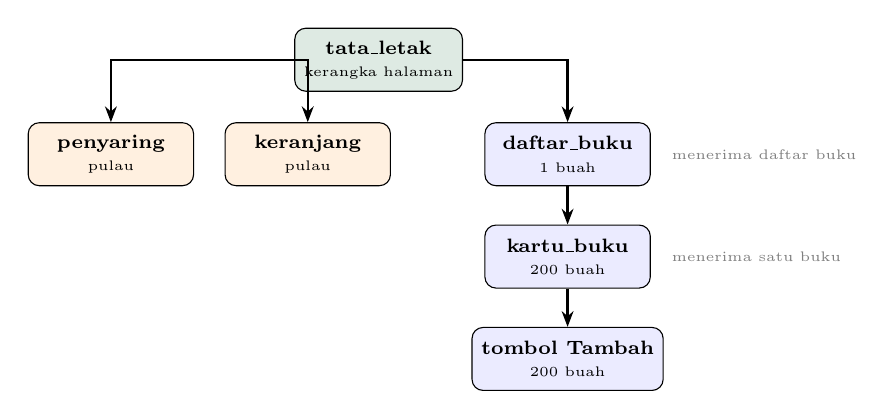
\begin{tikzpicture}[
    font=\scriptsize,
    kotak/.style={draw, rounded corners, minimum height=0.8cm,
                  minimum width=2.1cm, align=center, font=\scriptsize\bfseries},
    panah/.style={-{Stealth[length=2mm]}, thick}
  ]
    \node[kotak, fill=praditagreen!15] (halaman) at (0,2.1) {tata\_letak\\{\tiny\mdseries kerangka halaman}};
    \node[kotak, fill=orange!12] (penyaring) at (-3.4,0.9) {penyaring\\{\tiny\mdseries pulau}};
    \node[kotak, fill=orange!12] (keranjang) at (-0.9,0.9) {keranjang\\{\tiny\mdseries pulau}};
    \node[kotak, fill=blue!8] (daftar) at (2.4,0.9) {daftar\_buku\\{\tiny\mdseries 1 buah}};
    \node[kotak, fill=blue!8] (kartu) at (2.4,-0.4) {kartu\_buku\\{\tiny\mdseries 200 buah}};
    \node[kotak, fill=blue!8] (tombol) at (2.4,-1.7) {tombol Tambah\\{\tiny\mdseries 200 buah}};

    \draw[panah] (halaman) -| (penyaring);
    \draw[panah] (halaman) -| (keranjang);
    \draw[panah] (halaman) -| (daftar);
    \draw[panah] (daftar) -- (kartu);
    \draw[panah] (kartu) -- (tombol);
    \node[font=\tiny, gray, anchor=west] at (3.6,-0.4) {menerima satu buku};
    \node[font=\tiny, gray, anchor=west] at (3.6,0.9) {menerima daftar buku};
  \end{tikzpicture}
  \vspace{2pt}
  {\small Analoginya beton pracetak: tiap panel dicetak terpisah dengan
  ukuran yang sudah pasti, lalu dipasang di tempatnya.}
\end{frame}

\begin{frame}{{\Large 403 Komponen, Dua Pulau}}
  \vspace{12pt}
  \begin{itemize}
    \item Pada halaman 200 buku, \texttt{data-komponen} muncul \textbf{403}
          kali: satu daftar, 200 kartu, 200 tombol, satu penyaring, satu
          keranjang.
    \item \texttt{data-pulau} muncul \textbf{dua} kali, dan jumlah itu tidak
          berubah walaupun bukunya menjadi 2.000.
  \end{itemize}
  \vspace{10pt}
  {\small Karena tiap komponen menandai dirinya, jumlahnya dapat dihitung
  dengan satu perintah, dan biaya menghidupkannya dapat diukur.}
\end{frame}

\begin{frame}[fragile]{{\Large Komponen Terkecil: Satu Fungsi, Satu Buku}}
  \vspace{2pt}
\begin{lstlisting}[style=PythonStyle]
def kartu_buku(buku):
  judul = html.escape(buku["judul"])
  harga = f"Rp {buku['harga']:,}".replace(",", ".")
  alamat = f"/kerangka/buku/{buku['id']}"
  return (
      f'      <li class="kartu" data-komponen="kartu"'
      f' data-id="{buku["id"]}">\n'
      f'        <a class="judul" href="{alamat}">{judul}</a>\n'
      f'        <span class="harga">{harga}</span>\n'
      '        <button data-komponen="tombol" type="button">'
      "Tambah</button>\n"
      "      </li>"
  )
\end{lstlisting}
  \vspace{2pt}
  {\small Kartu tidak tahu ada berapa kartu lain di halaman yang sama.}
\end{frame}

\section{Design System dan Token}

\begin{frame}{\hfill}
  \centering
  \Huge{\textbf{Design System dan Token}}
\end{frame}

\begin{frame}[fragile]{{\Large Satu Sumber Nilai Tampilan}}
  \vspace{2pt}
\begin{lstlisting}[style=PythonStyle]
TOKEN = {
    "warna_utama": "#257147",
    "warna_teks": "#1a1a1a",
    "warna_garis": "#d8d8d8",
    "jarak_kecil": "4px",
    "jarak_sedang": "12px",
    "lebar_halaman": "720px",
}
\end{lstlisting}
  \vspace{2pt}
  {\small Analoginya satu kaleng cat untuk seluruh gedung. Mengubah satu
  baris di sini mengubah seluruh halaman, dan tidak ada tempat lain yang
  perlu dicari.}
\end{frame}

\begin{frame}{{\Large Token dan Tempat Pemakaiannya}}
  \vspace{6pt}
  \centering
  {\footnotesize
  \begin{tabularx}{\textwidth}{llY}
    \hline
    \textbf{Token} & \textbf{Nilai} & \textbf{Dipakai pada} \\
    \hline
    \texttt{warna\_utama} & \#257147 & judul buku \\
    \hline
    \texttt{warna\_teks} & \#1a1a1a & seluruh teks halaman \\
    \hline
    \texttt{warna\_garis} & \#d8d8d8 & garis tepi kartu \\
    \hline
    \texttt{jarak\_kecil} & 4px & jarak antarkartu \\
    \hline
    \texttt{jarak\_sedang} & 12px & jarak di dalam kartu \\
    \hline
    \texttt{lebar\_halaman} & 720px & lebar maksimum badan halaman \\
    \hline
  \end{tabularx}}
  \vspace{6pt}
  {\small Pada proyek besar, token inilah yang membuat dua tim yang bekerja
  terpisah tetap menghasilkan tampilan yang sama.}
\end{frame}

\section{Server State dan Client State}

\begin{frame}{\hfill}
  \centering
  \Huge{\textbf{Server State dan Client State}}
\end{frame}

\begin{frame}{{\Large Dua Jenis State yang Sering Tertukar}}
  \vspace{4pt}
  \centering
  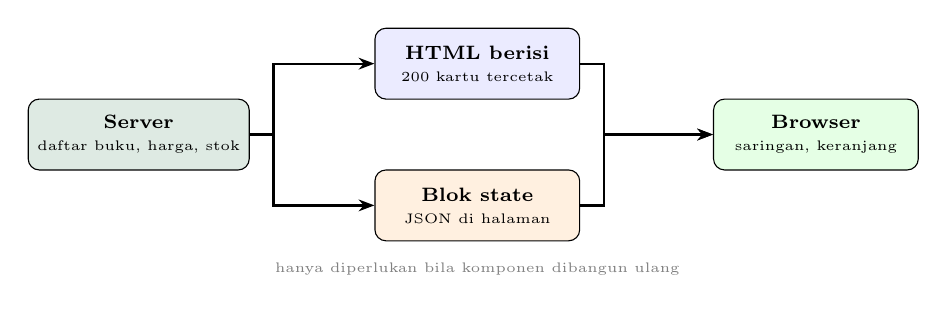
\begin{tikzpicture}[
    font=\scriptsize,
    kotak/.style={draw, rounded corners, minimum height=0.9cm,
                  minimum width=2.6cm, align=center, font=\scriptsize\bfseries},
    panah/.style={-{Stealth[length=2mm]}, thick}
  ]
    \node[kotak, fill=praditagreen!15] (server) at (0,0) {Server\\{\tiny\mdseries daftar buku, harga, stok}};
    \node[kotak, fill=blue!8] (html) at (4.3,0.9) {HTML berisi\\{\tiny\mdseries 200 kartu tercetak}};
    \node[kotak, fill=orange!12] (blok) at (4.3,-0.9) {Blok state\\{\tiny\mdseries JSON di halaman}};
    \node[kotak, fill=green!10] (browser) at (8.6,0) {Browser\\{\tiny\mdseries saringan, keranjang}};

    \draw[panah] (server.east) -- ++(0.3,0) |- (html.west);
    \draw[panah] (server.east) -- ++(0.3,0) |- (blok.west);
    \draw[panah] (html.east) -- ++(0.3,0) |- (browser.west);
    \draw[panah] (blok.east) -- ++(0.3,0) |- (browser.west);
    \node[font=\tiny, gray, anchor=north] at (4.3,-1.5) {hanya diperlukan bila komponen dibangun ulang};
  \end{tikzpicture}
  \vspace{4pt}
  {\small \textit{Server state} dimiliki server, dan browser memegang
  \textit{copy}-nya. \textit{Client state} lahir dan mati di browser.}
\end{frame}

\begin{frame}{{\Large Data yang Tiba Dua Kali}}
  \vspace{12pt}
  \begin{itemize}
    \item Pada hidrasi penuh, data buku tiba dua kali: sebagai HTML yang
          sudah tercetak, dan sebagai JSON di dalam blok \textit{state}.
    \item Halaman 200 buku tumbuh dari \textbf{55.674} byte menjadi
          \textbf{71.950} byte, naik 16.276 byte atau 29 persen.
    \item Angka keranjang disimpan di DOM wilayah, sehingga kembali ke nol
          begitu wilayahnya diganti.
  \end{itemize}
  \vspace{8pt}
  {\small \textit{State} yang harus bertahan melewati perpindahan tidak boleh
  tinggal di bagian yang ikut diganti.}
\end{frame}

\section{Server Component dan Client Component}

\begin{frame}{\hfill}
  \centering
  \Huge{\textbf{Server Component dan\\Client Component}}
\end{frame}

\begin{frame}{{\Large Siapa Dihidupkan, Siapa Tidak}}
  \vspace{6pt}
  \centering
  {\footnotesize
  \begin{tabularx}{\textwidth}{Ylll}
    \hline
    \textbf{Komponen} & \textbf{Jumlah} & \textbf{Hidrasi penuh} & \textbf{Hidrasi selektif} \\
    \hline
    kartu buku & 200 & dihidupkan & tidak \\
    \hline
    tombol Tambah & 200 & dihidupkan & tidak \\
    \hline
    daftar & 1 & dihidupkan & tidak \\
    \hline
    penyaring & 1 & dihidupkan & dihidupkan \\
    \hline
    keranjang & 1 & dihidupkan & dihidupkan \\
    \hline
    \textbf{Jumlah dihidupkan} & & \textbf{403} & \textbf{2} \\
    \hline
  \end{tabularx}}
  \vspace{6pt}
  {\small Varian penuh memasang 200 \textit{listener} di 200 tombol. Varian
  selektif memasang satu \textit{listener} di daftarnya. Perilakunya sama:
  dua klik menaikkan keranjang menjadi 2 pada keduanya.}
\end{frame}

\begin{frame}[fragile]{{\Large State yang Dikirim Kedua Varian}}
  \vspace{2pt}
\begin{lstlisting}[style=PythonStyle]
def state_penuh(daftar):
  return {
      "buku": {str(buku["id"]): buku for buku in daftar},
      "keranjang": 0,
      "saringan": "",
  }


def state_pulau():
  return {"keranjang": 0, "saringan": ""}
\end{lstlisting}
  \vspace{2pt}
  {\small Pulau tidak membangun ulang kartu, sehingga data kartu tidak
  diperlukan di browser.}
\end{frame}

\section{Hidrasi Penuh dan Hidrasi Selektif}

\begin{frame}{\hfill}
  \centering
  \Huge{\textbf{Hidrasi Penuh dan\\Hidrasi Selektif}}
\end{frame}

\begin{frame}{{\Large Jangkauan Hidrasi pada Halaman yang Sama}}
  \vspace{4pt}
  \centering
  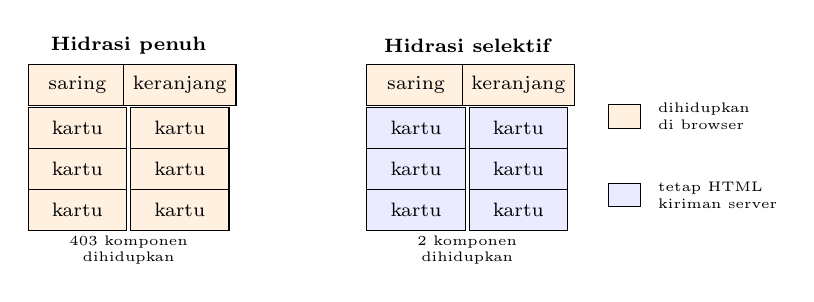
\begin{tikzpicture}[
    font=\scriptsize,
    sel/.style={draw, minimum height=0.52cm, minimum width=1.25cm},
    judul/.style={font=\scriptsize\bfseries, align=center},
    panah/.style={-{Stealth[length=2mm]}, thick}
  ]
    \node[judul] at (1.3,1.5) {Hidrasi penuh};
    \node[sel, fill=orange!12] at (0.65,1.0) {saring};
    \node[sel, fill=orange!12] at (1.95,1.0) {keranjang};
    \foreach \y in {0.45,-0.07,-0.59} {
      \node[sel, fill=orange!12] at (0.65,\y) {kartu};
      \node[sel, fill=orange!12] at (1.95,\y) {kartu};
    }
    \node[font=\tiny, align=center] at (1.3,-1.1) {403 komponen\\dihidupkan};

    \node[judul] at (5.6,1.5) {Hidrasi selektif};
    \node[sel, fill=orange!12] at (4.95,1.0) {saring};
    \node[sel, fill=orange!12] at (6.25,1.0) {keranjang};
    \foreach \y in {0.45,-0.07,-0.59} {
      \node[sel, fill=blue!8] at (4.95,\y) {kartu};
      \node[sel, fill=blue!8] at (6.25,\y) {kartu};
    }
    \node[font=\tiny, align=center] at (5.6,-1.1) {2 komponen\\dihidupkan};

    \node[sel, fill=orange!12, minimum width=0.4cm, minimum height=0.3cm] at (7.6,0.6) {};
    \node[font=\tiny, anchor=west, align=left] at (7.9,0.6) {dihidupkan\\di browser};
    \node[sel, fill=blue!8, minimum width=0.4cm, minimum height=0.3cm] at (7.6,-0.4) {};
    \node[font=\tiny, anchor=west, align=left] at (7.9,-0.4) {tetap HTML\\kiriman server};
  \end{tikzpicture}
\end{frame}

\begin{frame}[fragile]{{\Large Satu Baris Pembeda}}
  \vspace{2pt}
\begin{lstlisting}[language=TypeScript]
function hidrasiPenuh() {
  const mulai = performance.now();
  const state = bacaState();
  const daftar = document.querySelectorAll("[data-komponen]");
  for (const node of daftar) {
    hidupkanKomponen(node, state);
  }
  laporkan(daftar.length, performance.now() - mulai);
}
\end{lstlisting}
  \vspace{2pt}
  {\small \texttt{hidrasiSelektif()} sama persis, kecuali dua nama:
  \texttt{[data-komponen]} menjadi \texttt{[data-pulau]}, dan
  \texttt{hidupkanKomponen} menjadi \texttt{hidupkanPulau}. Halaman
  mengukur dirinya sendiri dengan \texttt{performance.now()}.}
\end{frame}

\begin{frame}{{\Large Biaya Hidrasi, Diukur}}
  \vspace{6pt}
  \centering
  {\footnotesize
  \begin{tabularx}{\textwidth}{Ylllll}
    \hline
    \textbf{Buku} & \textbf{Varian} & \textbf{Komponen} & \textbf{HTML byte} & \textbf{Tengah ms} & \textbf{Rentang ms} \\
    \hline
    200 & penuh & 403 & 71.950 & 1,50 & 1,20--2,10 \\
    \hline
    200 & selektif & 2 & 55.674 & 0,50 & 0,50--0,70 \\
    \hline
    1.000 & penuh & 2.003 & 358.360 & 3,90 & 3,60--4,70 \\
    \hline
    1.000 & selektif & 2 & 275.679 & 1,00 & 0,60--1,00 \\
    \hline
    2.000 & penuh & 4.003 & 722.356 & 7,10 & 6,30--10,40 \\
    \hline
    2.000 & selektif & 2 & 553.677 & 0,80 & 0,70--0,90 \\
    \hline
  \end{tabularx}}
  \vspace{6pt}
  {\small Lima kali pengukuran tiap varian, yang dicatat nilai tengahnya.}
\end{frame}

\begin{frame}{{\Large Dua Konsekuensi dan Satu Kejanggalan}}
  \vspace{10pt}
  \begin{itemize}
    \item Biaya hidrasi penuh tumbuh mengikuti jumlah komponen: 1,50 ms pada
          403 komponen, 7,10 ms pada 4.003 komponen.
    \item Biaya hidrasi selektif tidak bergerak dan tetap di bawah satu
          milidetik, karena yang dihidupkan tetap dua.
    \item Angka varian selektif bahkan tidak urut, yaitu 1,00 ms pada 1.000
          buku lalu 0,80 ms pada 2.000 buku. Biayanya sudah sekecil
          \textit{noise} pengukurannya.
  \end{itemize}
  \vspace{6pt}
  {\small Pada halaman 2.000 buku, blok \textit{state} tambahannya 168.679
  byte. Pada sambungan 1,5 Mbit per detik, byte sebanyak itu memakan sekitar
  0,9 detik sebelum satu baris skrip pun berjalan.}
\end{frame}

\section{Application Shell dan Routing}

\begin{frame}{\hfill}
  \centering
  \Huge{\textbf{Application Shell dan Routing}}
\end{frame}

\begin{frame}{{\Large Kerangka Tetap, Wilayahnya Diganti}}
  \vspace{4pt}
  \centering
  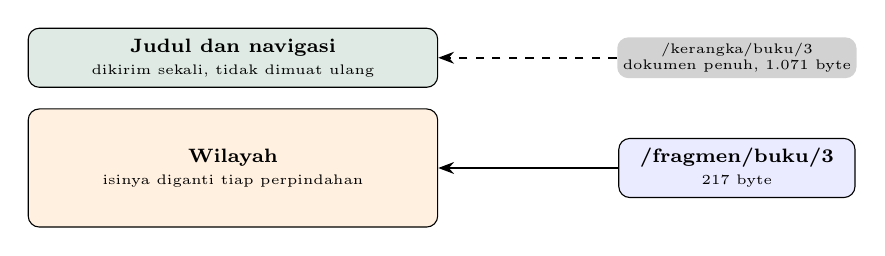
\begin{tikzpicture}[
    font=\scriptsize,
    kotak/.style={draw, rounded corners, minimum height=0.75cm,
                  minimum width=3.0cm, align=center, font=\scriptsize\bfseries},
    panah/.style={-{Stealth[length=2mm]}, thick}
  ]
    \node[kotak, fill=praditagreen!15, minimum width=5.2cm] (judul) at (0,1.5) {Judul dan navigasi\\{\tiny\mdseries dikirim sekali, tidak dimuat ulang}};
    \node[kotak, fill=orange!12, minimum width=5.2cm, minimum height=1.5cm] (wilayah) at (0,0.1) {Wilayah\\{\tiny\mdseries isinya diganti tiap perpindahan}};
    \node[kotak, fill=blue!8] (fragmen) at (6.4,0.1) {/fragmen/buku/3\\{\tiny\mdseries 217 byte}};
    \node[font=\tiny, align=center, fill=gray!35, rounded corners, inner sep=2pt] (dokumen) at (6.4,1.5) {/kerangka/buku/3\\dokumen penuh, 1.071 byte};

    \draw[panah] (fragmen) -- (wilayah);
    \draw[panah, dashed] (dokumen.west) -- ++(-0.5,0) |- (judul.east);
  \end{tikzpicture}
  \vspace{2pt}
  {\small Analoginya ruang kuliah dengan satu papan tulis: dinding dan
  mejanya tidak dibongkar tiap kali mata kuliahnya berganti.}
\end{frame}

\begin{frame}{{\Large Dokumen lawan Fragmen, Diukur}}
  \vspace{6pt}
  \centering
  {\footnotesize
  \begin{tabularx}{\textwidth}{Yllll}
    \hline
    \textbf{Tujuan} & \textbf{Status} & \textbf{Dokumen} & \textbf{Fragmen} & \textbf{Fragmen \%} \\
    \hline
    \texttt{/katalog} & 200 & 55.943 & 55.089 & 98,5 \\
    \hline
    \texttt{/katalog?saring=jaringan} & 200 & 10.414 & 9.560 & 91,8 \\
    \hline
    \texttt{/buku/3} & 200 & 1.071 & 217 & 20,3 \\
    \hline
    \texttt{/gagal} & 500 & 1.023 & 169 & 16,5 \\
    \hline
  \end{tabularx}}
  \vspace{6pt}
  {\small Baris pertama dibiarkan apa adanya walaupun melawan harapan:
  fragmen katalog 98,5 persen sebesar dokumennya, karena yang dituju memang
  hampir seluruh halaman.}
\end{frame}

\begin{frame}{{\Large Yang Sebenarnya Dihemat}}
  \vspace{10pt}
  \begin{itemize}
    \item Penghematan byte baru terasa pada tujuan yang kecil: fragmen satu
          buku 217 byte, dokumennya 1.071 byte.
    \item Dokumen juga membawa kerangka, gaya, dan rujukan ke
          \texttt{rute.js} sebesar 4.188 byte yang harus diurai ulang.
    \item Perpindahan lewat fragmen tidak menyentuh satu pun dari ketiganya,
          dan penghematan itu tidak muncul di kolom byte.
  \end{itemize}
  \vspace{6pt}
  {\small Diperiksa di browser: tautan mengganti isi wilayah tanpa memuat
  ulang dokumen, alamat berubah menjadi \texttt{/kerangka/buku/3}, dan tombol
  kembali browser memulihkan katalog beserta 200 barisnya.}
\end{frame}

\section{Batas Error dan Progressive Enhancement}

\begin{frame}{\hfill}
  \centering
  \Huge{\textbf{Batas Error dan\\Progressive Enhancement}}
\end{frame}

\begin{frame}[fragile]{{\Large Dua Kegagalan Diperiksa Sekaligus}}
  \vspace{2pt}
\begin{lstlisting}[language=TypeScript]
async function muatWilayah(alamat) {
  try {
    const respon = await fetch(alamatFragmen(alamat));
    if (!respon.ok) {
      tampilkanGagal(PESAN_GAGAL);
      return;
    }
    document.getElementById("wilayah").innerHTML = await respon.text();
  } catch (gagal) {
    tampilkanGagal(PESAN_GAGAL);
  }
}
\end{lstlisting}
  \vspace{2pt}
  {\small \texttt{fetch} tidak menganggap status 500 sebagai kegagalan.
  Tanpa pemeriksaan status, halaman \textit{error} akan terpasang seolah-olah
  isi yang benar.}
\end{frame}

\begin{frame}{{\Large Apa yang Tersisa Tanpa Skrip}}
  \vspace{6pt}
  \centering
  {\footnotesize
  \begin{tabularx}{\textwidth}{Ylll}
    \hline
    \textbf{Halaman} & \textbf{Skrip jalan} & \textbf{Skrip mati} & \textbf{Form} \\
    \hline
    \texttt{/selektif} & 200 baris & 200 baris & ada \\
    \hline
    \texttt{/selektif?saring=jaringan} & 33 baris & 33 baris & ada \\
    \hline
    \texttt{/kerangka/katalog} & 200 baris & 200 baris & ada \\
    \hline
    \texttt{/kerangka/katalog?saring=jaringan} & 33 baris & 33 baris & ada \\
    \hline
  \end{tabularx}}
  \vspace{6pt}
  {\small Kedua kolom angkanya sama, dan kesamaan itulah hasilnya: tidak ada
  satu baris katalog pun yang bergantung pada skrip. Pengujiannya memakai CSP
  penolak skrip, seperti ketika file JavaScript-nya gagal diunduh.}
\end{frame}

\begin{frame}{{\Large Aksesibilitas Didapat dari HTML-nya}}
  \vspace{10pt}
  \begin{itemize}
    \item Tombol Tambah adalah \texttt{<button>} sungguhan, sehingga dapat
          dicapai dengan Tab dan ditekan dengan spasi.
    \item Kotak penyaring punya \texttt{<label for>}, sehingga pembaca layar
          menyebutkan namanya.
    \item Tautan navigasi adalah \texttt{<a href>} beralamat sungguhan,
          sehingga dapat dibuka di tab baru walaupun routernya ada.
    \item Wilayah yang isinya berubah ditandai
          \texttt{aria-live="polite"}, agar penggantiannya diberitakan.
  \end{itemize}
\end{frame}

\section{Persiapan Latihan}

\begin{frame}{\hfill}
  \centering
  \Huge{\textbf{Persiapan Latihan}}
\end{frame}

\begin{frame}[fragile]{{\Large Satu Perintah}}
  \vspace{2pt}
\begin{lstlisting}[language=bash]
cd sources/chapter11
python3 aplikasi.py &

# Keluarannya:
# Melayani di http://127.0.0.1:8080/penuh dengan 200 buku
\end{lstlisting}
  \vspace{4pt}
  {\small Latihan membutuhkan Python 3 dan satu browser berbasis Chromium,
  tanpa Docker dan tanpa pustaka tambahan. Seluruh permintaan diarahkan ke
  aplikasi di komputer sendiri, dan sifatnya mengamati, bukan membebani.}
\end{frame}

\section{Latihan 1: Komponen dan State}

\begin{frame}{\hfill}
  \centering
  \Huge{\textbf{Latihan 1:\\Komponen dan State}}
\end{frame}

\begin{frame}[fragile]{{\Large Menghitung Komponen dan Ukuran Halaman}}
  \vspace{2pt}
\begin{lstlisting}[language=bash]
curl -s http://127.0.0.1:8080/penuh | grep -c 'data-komponen='
curl -s http://127.0.0.1:8080/selektif | grep -c 'data-pulau='
curl -s http://127.0.0.1:8080/penuh | wc -c
curl -s http://127.0.0.1:8080/selektif | wc -c

# Keluarannya:
# 403
# 2
# 71950
# 55674
\end{lstlisting}
  \vspace{2pt}
  {\small Ulangi dengan \texttt{JUMLAH\_BUKU=1000}, lalu jawab: berapa persen
  tambahan ukuran HTML pada varian penuh, dan dari mana asalnya?}
\end{frame}

\section{Latihan 2: Biaya Hidrasi}

\begin{frame}{\hfill}
  \centering
  \Huge{\textbf{Latihan 2:\\Biaya Hidrasi}}
\end{frame}

\begin{frame}[fragile]{{\Large Mengukur Kedua Varian}}
  \vspace{2pt}
\begin{lstlisting}[language=bash]
python3 ukur-hidrasi.py

# Keluarannya:
#   Varian     Buku  Komponen  HTML byte  JS byte  Tengah ms   Rentang ms
#   penuh       200       403      71950     3723       1.50    1.20-2.10
#   selektif    200         2      55674     3278       0.50    0.50-0.70
\end{lstlisting}
  \vspace{2pt}
  {\small Ulangi pada \texttt{JUMLAH\_BUKU=1000} dan
  \texttt{JUMLAH\_BUKU=2000}, lalu jawab: bagian mana yang tumbuh mengikuti
  besar halaman, dan mengapa angka varian selektif tidak urut?}
\end{frame}

\begin{frame}{{\Large Lembar Isian Latihan 2}}
  \vspace{6pt}
  \centering
  {\footnotesize
  \begin{tabularx}{\textwidth}{Yllll}
    \hline
    \textbf{Buku} & \textbf{Penuh, ms} & \textbf{Selektif, ms} & \textbf{Komponen penuh} & \textbf{Pulau} \\
    \hline
    200 & \dots & \dots & \dots & \dots \\
    \hline
    1.000 & \dots & \dots & \dots & \dots \\
    \hline
    2.000 & \dots & \dots & \dots & \dots \\
    \hline
  \end{tabularx}}
  \vspace{6pt}
  {\small Angka milidetik tiap mahasiswa akan berbeda, karena bergantung pada
  komputernya. Yang dilaporkan pola perbandingannya, bukan angka persisnya.}
\end{frame}

\section{Latihan 3: Biaya Perpindahan}

\begin{frame}{\hfill}
  \centering
  \Huge{\textbf{Latihan 3:\\Biaya Perpindahan}}
\end{frame}

\begin{frame}[fragile]{{\Large Dokumen lawan Fragmen}}
  \vspace{2pt}
\begin{lstlisting}[language=bash]
python3 ukur-rute.py

# Keluarannya:
#   Tujuan                    Status   Dokumen   Fragmen  Fragmen %
#   /katalog                 200/200     55943     55089      98.5%
#   /katalog?saring=jaringan 200/200     10414      9560      91.8%
#   /buku/3                  200/200      1071       217      20.3%
#   /gagal                   500/500      1023       169      16.5%
\end{lstlisting}
  \vspace{2pt}
  {\small Lalu di browser: buka \texttt{/kerangka/katalog}, tekan tautan
  "Buku 3", tekan tombol kembali, dan tekan Tambah dua kali sebelum
  berpindah. Catat angka keranjang sesudah kembali.}
\end{frame}

\section{Latihan 4: Tanpa Skrip}

\begin{frame}{\hfill}
  \centering
  \Huge{\textbf{Latihan 4:\\Tanpa Skrip}}
\end{frame}

\begin{frame}[fragile]{{\Large Memeriksa Isi Tanpa Skrip}}
  \vspace{2pt}
\begin{lstlisting}[language=bash]
python3 ukur-tanpa-js.py

# Keluarannya:
#   Halaman                            Skrip jalan Skrip mati  Form
#   /selektif                                  200        200   ada
#   /selektif?saring=jaringan                   33         33   ada
#   /kerangka/katalog                          200        200   ada
#   /kerangka/katalog?saring=jaringan           33         33   ada
\end{lstlisting}
  \vspace{2pt}
  {\small Lalu buka \texttt{/kerangka/katalog?blokir\_skrip=1}, saring
  "jaringan", dan bandingkan dengan halaman yang skripnya jalan. Tekan juga
  tautan "Bagian yang gagal", lalu catat navigasinya masih utuh atau tidak.}
\end{frame}

\section{Ringkasan}

\begin{frame}{\hfill}
  \centering
  \Huge{\textbf{Ringkasan}}
\end{frame}

\begin{frame}{{\Large Ringkasan}}
  \vspace{8pt}
  \begin{itemize}
    \item Komponen dan token mengatur kode, bukan biaya. Batas yang jelas
          membuat halaman dapat dihitung: 403 komponen dan dua pulau.
    \item Hidrasi penuh menghidupkan 403 komponen dalam 1,50 ms, dan 4.003
          komponen dalam 7,10 ms. Hidrasi selektif tetap di 0,50 sampai 1,00
          ms, berapa pun bukunya.
    \item Selisih yang lebih mudah dirasakan ada di ukuran halaman: 168.679
          byte tambahan pada 2.000 buku, atau 30 persen lebih besar.
    \item Kerangka aplikasi memisahkan yang tetap dari yang berganti, tetapi
          penghematannya tidak selalu besar: fragmen katalog 98,5 persen
          sebesar dokumennya.
    \item Urutan membangunnya yang menentukan: HTML yang sudah berfungsi
          paling bawah, skrip hanya pada bagian yang memang butuh hidup.
  \end{itemize}
\end{frame}

\end{document}
